\documentclass[tikz]{standalone}
\usepackage{xcolor}

\begin{document}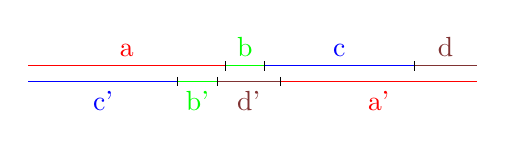
\begin{tikzpicture}
\definecolor{cola}{rgb}{1,0,0};
\definecolor{colb}{rgb}{0,1,0};
\definecolor{colc}{rgb}{0,0,1};
\definecolor{cold}{rgb}{.5,.2,.2};

\coordinate (la) at (2.5,0);
\coordinate (lb) at (.5,0);
\coordinate (lc) at (1.9,0);
\coordinate (ld) at (.8,0);

% top 1
\draw[cola] (0,.1) ++(0,0) -- node[above] {a} +(la);
\draw[colb] (0,.1) ++(2.5,0) -- node[above] {b} +(lb);
\draw[colc] (0,.1) ++(3,0) -- node[above] {c} +(lc);
\draw[cold] (0,.1) ++(4.9,0) -- node[above] {d} +(ld);

% bot 1
\draw[colc] (0,-.1) ++(0,0) -- node[below] {c'} +(lc);
\draw[colb] (0,-.1) ++(1.9,0) -- node[below] {b'} +(lb);
\draw[cold] (0,-.1) ++(2.4,0) -- node[below] {d'} +(ld);
\draw[cola] (0,-.1) ++(3.2,0) -- node[below] {a'} +(la);

% top cuts
\foreach \x in {2.5,3,4.9}
  \draw[black] +(\x,.04) -- +(\x,.16);
% bot cuts
\foreach \x in {1.9,2.4,3.2}
  \draw[black] +(\x,-.04) -- +(\x,-.16);
\end{tikzpicture}\end{document}
